\documentclass[class=article, crop=false]{standalone}
\usepackage{my_preamble}
\begin{document}
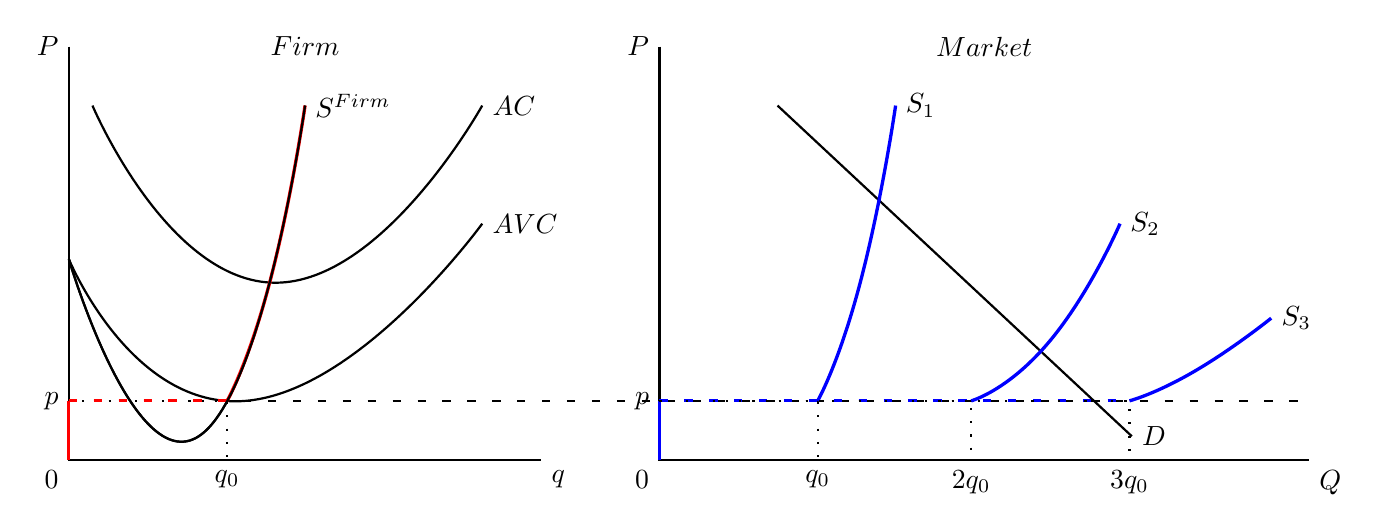
\begin{tikzpicture}[thick,font=\sffamily,scale=1.5]
	%axis and labels
	\draw (0,3.5) node[left]{$P$} -- (0,0) node[below left] {$0$} -- (4,0) node[below right]{$q$};
	\draw (5,3.5) node[left]{$P$} -- (5,0) node[below left] {$0$} -- (10.5,0) node[below right]{$Q$};
	\node[] at (2,3.5) {$Firm$}; %Firm label  
	\node[] at (7.75,3.5) {$Market$}; %Market label  
	
	%Firm--------------------------------------
		%graphs	
		\draw[] plot [smooth, tension=1] coordinates {(0.2,3) (1.75,1.5) (3.5,3)}; %AC
		\draw[] plot [smooth, tension=1] coordinates {(0,1.7) (1.5,0.5) (3.5,2)}; %AVC
		\draw[] plot [smooth, tension=1] coordinates {(0,1.7) (1.1,0.2) (2,3)}; %MC
		
		%dotted lines
		\draw[loosely dotted] (0,0.5) node[left]{$p$} -| node[pos=0.25,below=3mm] {} (1.34,0) node[below]{$q_{0}$}; %Dotted lines
		\draw[loosely dashed] (0,0.5) -- (10.5,0.5); %p line
		
		%Firm supply curve	
		\draw[very thick, red] (0,0) -- (0,0.5); %part 1
		\draw[very thick, red, loosely dashed] (0,0.5)--(1.34, 0.5); %part 2
		\draw[very thick, red] plot [smooth, tension=1] coordinates{(1.34, 0.5) (1.7,1.5) (2,3)}; %part 3
	
		%labels
		\node[right] at (2,3) {$S^{Firm}$}; %firm supply label 
		\node[right] at (3.5,3) {$AC$}; %AC label 
		\node[right] at (3.5,2) {$AVC$}; %AVC label
		\draw[] plot [smooth, tension=1] coordinates {(0,1.7) (1.1,0.2) (2,3)}; %MC
	
	%Market------------------------------------
		\draw[] (6,3) -- (9,0.2); %Demand
		
				
		%Market supply curve	
		\draw[very thick, blue] (5,0) -- (5,0.5); %part 1
		\draw[very thick, blue, loosely dashed] (5,0.5)--(9, 0.5); %part 2
		\draw[very thick, blue] plot [smooth, tension=1] coordinates{(6.34, 0.5) (6.7,1.5) (7,3)}; %part 3a
		\draw[very thick, blue] plot [smooth, tension=1] coordinates{(7.64,0.5) (8.3,1) (8.9,2)}; %part 3b
		\draw[very thick, blue] plot [smooth, tension=1] coordinates{(8.98, 0.5) (9.53,0.75) (10.18,1.2)}; %part 3c
		
		%dotted lines
		\draw[loosely dotted] (5,0.5) node[left]{$p$} -| node[pos=0.25,below=3mm] {} (6.34,0) node[below]{$q_{0}$}; %Dotted lines 1
		\draw[loosely dotted] (5,0.5) node[left]{} -| node[pos=0.25,below=3mm] {} (7.64,0) node[below]{$2q_{0}$}; %Dotted lines 2
		\draw[loosely dotted] (5,0.5) node[left]{} -| node[pos=0.25,below=3mm] {} (8.98,0) node[below]{$3q_{0}$}; %Dotted lines 3
		
		%labels
		\node[right] at (9,0.2) {$D$}; %Demand supply label  
		\node[right] at (7,3) {$S_{1}$}; %SR1 supply label  
		\node[right] at (8.9,2) {$S_{2}$}; %SR2 supply label  
		\node[right] at (10.18,1.2) {$S_{3}$}; %SR3 supply label  
\end{tikzpicture}
\end{document}